% Chapter Template

\chapter{Basic Principles}
\label{Chapter2:Background} 

In this chapter we will discuss the basic  principles needed for this work. The entire chapter is divided into two sections. In the first chapter we will go through some theory of neural network and basic building blocks  needed for designing a proper neural network for the depth estimation task, most of the concepts are taken from Friedman et al. \cite{friedman2001elements}. Second part will be comprising of some basics of depth estimation and camera parameters concepts. Since the area of Artificial Neural Network is very vast we will be focusing on the concepts which was specifically used for this study. 

\section{Artificial Neural Networks}

As we know Artificial Neural Networks (ANNs) are a developed similar to brain style computation consisting of different level of neurons. In other words we can say its a statistical learning or science of learning from given data. There are various types of learning approaches for solving problems
regarding optimization \cite{friedman2001elements}. However, deep learning methodologies have proven to be favorable in ANNs and computer vision tasks such as classifying objects within images and in our we will be using Deep Convolutions Networks. 

To understand the basic types of Neural Network are supervised learning and Unsupervised learning. In general we denote \(X\) as input and \(Y\) as output of a given function. Supervised learning is when there is a labels \(y_{i}\) for each input example \(x_{i}\) where    \(\{(x_{1},y_{1}),(x_{2},y_{2}),...(x_{n},y_{n})\} \in X\) for a learning algorithm satisfying function \(f:X \rightarrow Y\) and output \( \hat{y_{i}} = P (y_{i}|x_{i})\). All labeled classification problems can be categorized under supervised learning such that. For  unsupervised learning clustering or grouping is the detection of similarities for a given input examples \({(x_{1},x_{2},...,x_{n})} \in X\) and joint density \(Pr(X)\)  where as in supervised learning \(Pr(X)\) is of no concern. In supervised learning there is a definite score of success because is \(P(y|y)\) \cite{friedman2001elements}. 

To discuss more about supervised learning with the help of simple binary logistic regression model is given by
\begin{equation} \label{eq1}
    \hat{y_{i}} = x_{i}W + b 
\end{equation}
The problem of this above equation is it linmited to 

%where b \in\mathbb{R}

\begin{equation} \label{eq2}
    e^{\pi i} + 1 = 0
\end{equation}

The basic nuts and bolts of NNs are ...

\section{Depth Estimation}
3D Scanning have become more and more important with emerging technology of Augmented Reality and Virtual Reality. These 3D scanners use different approaches to estimate the depth out of a scene. Some of the major approaches being used are Stereo Imaging, Structured Light System(SLS), Structure from Motion(SfM), Time of Flight(ToF) and Laser Triangulation. These approaches either use single frame or multiple frame to generate the third dimension Depth. For example, SfM takes multiple frames and with different views of the object to determine the depth. This not only needs heavy computation but is time consuming as well.On the other hand, Stereo Imaging only needs two frames with a Disparity map to calculate the Depth of objects.\\

\begin{figure}[h]
    \centering
    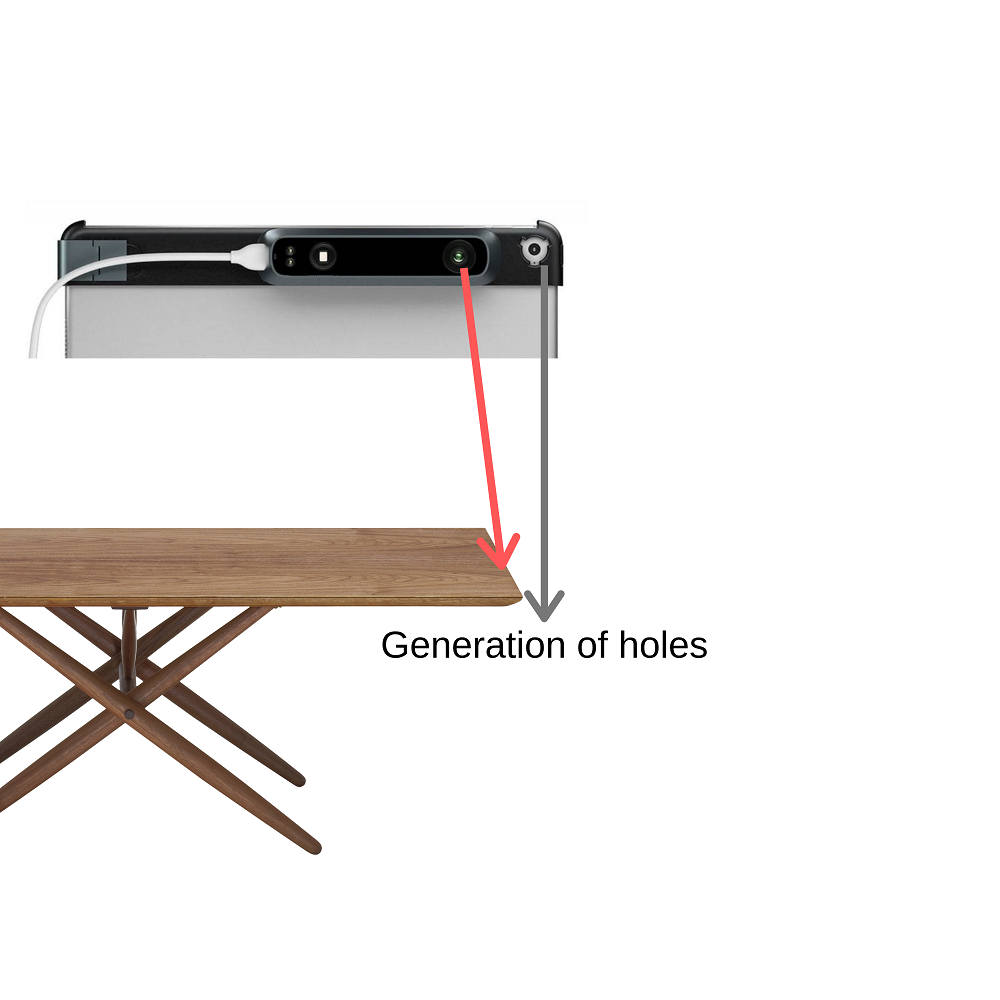
\includegraphics[scale=0.4]{Figures/holes.png}
    \caption{Generation of holes due to parallax}
    \label{fig:holes}
\end{figure}


ToF cameras work dynamically through the scene. They scan the environment using illuminating it with incoherent light. To measure the depth, the time taken by the light to reflect back to the sensor is noted. Although, ToF cameras are fast, they are often not accurate. The comparison between these techniques can also be seen in \ref{table:3DScanning} .These techniques are now widely being used to produce 3D scanners. For example Microsoft Kinect V2.0 uses ToF technique, while Structure Sensor by Occipital uses SLS. The comparison is discussed later in Chapter \ref{Chapter4:Dataset}.\\

\begin{table}[h]
\begin{tabular}{@{}lll@{}}
\toprule
\textbf{Technique}                    & \textbf{Advantage}           & \textbf{Disadvantage}         \\ \midrule
Structure from Motion          & High capture frequency & Time consuming                 \\
Time of Flight       & No effect of lighting & Low capture frequency     \\
Structured Light System        & High resolution   & Prone to noise                 \\ 
                            &                     &                                               
\end{tabular}
\caption{Comparison of different 3D Scanning Techniques}
\label{table:3DScanning}
\end{table}


Structure Sensor consist of a laser-emitting diode, infrared radiation range projector and an infrared sensor to sense the projected radiation. The infrared sensor records the reflecting intensity of the infrared (IR) light pattern projected by the IR projector onto the target while its  SOC triangulates the 3D scene. \cite{Kalantari} While these sensors are great devices they have some limitations. The distance they can measure is limited and they suffer from reflection problems on transparent, shiny, or very matte and absorbing objects. Another limitation is holes generated by parallax effect happening due to difference in position of the camera of Ipad and structure sensor.\\



In simpler terms, it works like human eyes. If we close one eye and then other, we notice a disparity. When there is an object we try to focus on, we see it through different angles. If the object is close enough, then sometimes one eye can see what is behind and other can not. This can be seen in figure \ref{fig:holes}. As a result, it produces a shadow of holes which can be seen in figure \ref{fig:holes2}\\


\begin{figure}[b]
    
\includegraphics[scale=0.29]{Figures/RGB.png} 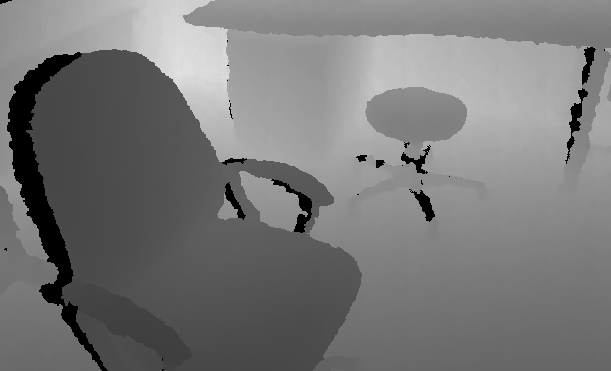
\includegraphics[scale=0.37]{Figures/Depth.png}
    \caption{Holes produced in depth image}
    \label{fig:holes2}
\end{figure}
